% Options for packages loaded elsewhere
\PassOptionsToPackage{unicode}{hyperref}
\PassOptionsToPackage{hyphens}{url}
%
\documentclass[
]{book}
\usepackage{lmodern}
\usepackage{amssymb,amsmath}
\usepackage{ifxetex,ifluatex}
\ifnum 0\ifxetex 1\fi\ifluatex 1\fi=0 % if pdftex
  \usepackage[T1]{fontenc}
  \usepackage[utf8]{inputenc}
  \usepackage{textcomp} % provide euro and other symbols
\else % if luatex or xetex
  \usepackage{unicode-math}
  \defaultfontfeatures{Scale=MatchLowercase}
  \defaultfontfeatures[\rmfamily]{Ligatures=TeX,Scale=1}
\fi
% Use upquote if available, for straight quotes in verbatim environments
\IfFileExists{upquote.sty}{\usepackage{upquote}}{}
\IfFileExists{microtype.sty}{% use microtype if available
  \usepackage[]{microtype}
  \UseMicrotypeSet[protrusion]{basicmath} % disable protrusion for tt fonts
}{}
\makeatletter
\@ifundefined{KOMAClassName}{% if non-KOMA class
  \IfFileExists{parskip.sty}{%
    \usepackage{parskip}
  }{% else
    \setlength{\parindent}{0pt}
    \setlength{\parskip}{6pt plus 2pt minus 1pt}}
}{% if KOMA class
  \KOMAoptions{parskip=half}}
\makeatother
\usepackage{xcolor}
\IfFileExists{xurl.sty}{\usepackage{xurl}}{} % add URL line breaks if available
\IfFileExists{bookmark.sty}{\usepackage{bookmark}}{\usepackage{hyperref}}
\hypersetup{
  pdftitle={Laboratório de Sistemas de Controle},
  pdfauthor={Djonathan Luiz de Oliveira Quadras},
  hidelinks,
  pdfcreator={LaTeX via pandoc}}
\urlstyle{same} % disable monospaced font for URLs
\usepackage{color}
\usepackage{fancyvrb}
\newcommand{\VerbBar}{|}
\newcommand{\VERB}{\Verb[commandchars=\\\{\}]}
\DefineVerbatimEnvironment{Highlighting}{Verbatim}{commandchars=\\\{\}}
% Add ',fontsize=\small' for more characters per line
\usepackage{framed}
\definecolor{shadecolor}{RGB}{248,248,248}
\newenvironment{Shaded}{\begin{snugshade}}{\end{snugshade}}
\newcommand{\AlertTok}[1]{\textcolor[rgb]{0.94,0.16,0.16}{#1}}
\newcommand{\AnnotationTok}[1]{\textcolor[rgb]{0.56,0.35,0.01}{\textbf{\textit{#1}}}}
\newcommand{\AttributeTok}[1]{\textcolor[rgb]{0.77,0.63,0.00}{#1}}
\newcommand{\BaseNTok}[1]{\textcolor[rgb]{0.00,0.00,0.81}{#1}}
\newcommand{\BuiltInTok}[1]{#1}
\newcommand{\CharTok}[1]{\textcolor[rgb]{0.31,0.60,0.02}{#1}}
\newcommand{\CommentTok}[1]{\textcolor[rgb]{0.56,0.35,0.01}{\textit{#1}}}
\newcommand{\CommentVarTok}[1]{\textcolor[rgb]{0.56,0.35,0.01}{\textbf{\textit{#1}}}}
\newcommand{\ConstantTok}[1]{\textcolor[rgb]{0.00,0.00,0.00}{#1}}
\newcommand{\ControlFlowTok}[1]{\textcolor[rgb]{0.13,0.29,0.53}{\textbf{#1}}}
\newcommand{\DataTypeTok}[1]{\textcolor[rgb]{0.13,0.29,0.53}{#1}}
\newcommand{\DecValTok}[1]{\textcolor[rgb]{0.00,0.00,0.81}{#1}}
\newcommand{\DocumentationTok}[1]{\textcolor[rgb]{0.56,0.35,0.01}{\textbf{\textit{#1}}}}
\newcommand{\ErrorTok}[1]{\textcolor[rgb]{0.64,0.00,0.00}{\textbf{#1}}}
\newcommand{\ExtensionTok}[1]{#1}
\newcommand{\FloatTok}[1]{\textcolor[rgb]{0.00,0.00,0.81}{#1}}
\newcommand{\FunctionTok}[1]{\textcolor[rgb]{0.00,0.00,0.00}{#1}}
\newcommand{\ImportTok}[1]{#1}
\newcommand{\InformationTok}[1]{\textcolor[rgb]{0.56,0.35,0.01}{\textbf{\textit{#1}}}}
\newcommand{\KeywordTok}[1]{\textcolor[rgb]{0.13,0.29,0.53}{\textbf{#1}}}
\newcommand{\NormalTok}[1]{#1}
\newcommand{\OperatorTok}[1]{\textcolor[rgb]{0.81,0.36,0.00}{\textbf{#1}}}
\newcommand{\OtherTok}[1]{\textcolor[rgb]{0.56,0.35,0.01}{#1}}
\newcommand{\PreprocessorTok}[1]{\textcolor[rgb]{0.56,0.35,0.01}{\textit{#1}}}
\newcommand{\RegionMarkerTok}[1]{#1}
\newcommand{\SpecialCharTok}[1]{\textcolor[rgb]{0.00,0.00,0.00}{#1}}
\newcommand{\SpecialStringTok}[1]{\textcolor[rgb]{0.31,0.60,0.02}{#1}}
\newcommand{\StringTok}[1]{\textcolor[rgb]{0.31,0.60,0.02}{#1}}
\newcommand{\VariableTok}[1]{\textcolor[rgb]{0.00,0.00,0.00}{#1}}
\newcommand{\VerbatimStringTok}[1]{\textcolor[rgb]{0.31,0.60,0.02}{#1}}
\newcommand{\WarningTok}[1]{\textcolor[rgb]{0.56,0.35,0.01}{\textbf{\textit{#1}}}}
\usepackage{longtable,booktabs}
% Correct order of tables after \paragraph or \subparagraph
\usepackage{etoolbox}
\makeatletter
\patchcmd\longtable{\par}{\if@noskipsec\mbox{}\fi\par}{}{}
\makeatother
% Allow footnotes in longtable head/foot
\IfFileExists{footnotehyper.sty}{\usepackage{footnotehyper}}{\usepackage{footnote}}
\makesavenoteenv{longtable}
\usepackage{graphicx,grffile}
\makeatletter
\def\maxwidth{\ifdim\Gin@nat@width>\linewidth\linewidth\else\Gin@nat@width\fi}
\def\maxheight{\ifdim\Gin@nat@height>\textheight\textheight\else\Gin@nat@height\fi}
\makeatother
% Scale images if necessary, so that they will not overflow the page
% margins by default, and it is still possible to overwrite the defaults
% using explicit options in \includegraphics[width, height, ...]{}
\setkeys{Gin}{width=\maxwidth,height=\maxheight,keepaspectratio}
% Set default figure placement to htbp
\makeatletter
\def\fps@figure{htbp}
\makeatother
\setlength{\emergencystretch}{3em} % prevent overfull lines
\providecommand{\tightlist}{%
  \setlength{\itemsep}{0pt}\setlength{\parskip}{0pt}}
\setcounter{secnumdepth}{5}
\usepackage{booktabs}
\usepackage[]{natbib}
\bibliographystyle{apalike}

\title{Laboratório de Sistemas de Controle}
\author{Djonathan Luiz de Oliveira Quadras}
\date{2020-05-27}

\begin{document}
\maketitle

{
\setcounter{tocdepth}{1}
\tableofcontents
}
\hypertarget{apresentauxe7uxe3o}{%
\chapter*{Apresentação}\label{apresentauxe7uxe3o}}
\addcontentsline{toc}{chapter}{Apresentação}

Working on it :)

\hypertarget{simulauxe7uxe3o-de-sistemas}{%
\chapter{Simulação de Sistemas}\label{simulauxe7uxe3o-de-sistemas}}

Este laboratório consistiu apenas na apresentação da disciplina, da ferramenta e do método que será aplicado. Não teve nehuma atividade desenvolvida.

\hypertarget{efeitos-de-puxf3los-e-zeros-na-dinuxe2mica}{%
\chapter{Efeitos de Pólos e Zeros na Dinâmica}\label{efeitos-de-puxf3los-e-zeros-na-dinuxe2mica}}

\hypertarget{apresentauxe7uxe3o-do-laboratuxf3rio}{%
\section{Apresentação do Laboratório}\label{apresentauxe7uxe3o-do-laboratuxf3rio}}

\hypertarget{objetivo}{%
\subsection{Objetivo}\label{objetivo}}

Nesta experiência, verificaremos a influência dos pólos e zeros de uma Função de Transferência na resposta dinâmica para entradas do tipo degrau e também para entradas senoidais. Utilizaremos o Matlab para realizar as
simulações.

\hypertarget{polos-e-zeros}{%
\subsection{Polos e Zeros}\label{polos-e-zeros}}

Considere uma função de Trasnferência da forma

\[
G(s) = \frac{Y(s)}{U(s)} = \frac{N(s)}{D(s)} = \frac{b_1s^m +b_2s^{m-1} + \dots + b_ms + b_{m+1}}{s^n + a_1s^{n-1}+ \dots + a_{n-1}s + a_n}
\]

onde \(Y(s)\) é a saída, \(U(s)\) é a entrada, \(n \geq m\) e todos os coeficientes são reais. Temos as seguintes definições:

\begin{enumerate}
\def\labelenumi{\arabic{enumi}.}
\tightlist
\item
  Os pólos \(G(s)\) são as raízes de \(D(s)\) (\(D(s) = 0\));
\item
  Os \emph{zeros} de \(G(s)\) são as raízes de \(N(s)\) (\(N(s) = 0\));
\item
  \(G(s)\) é \emph{estável} quando todos os pólos possuem parte real negativa, ou seja, estão no semi-plano esquerdo (SPE) do plano \(s\);
\item
  \(G(s)\) é \emph{instável} quando existe ao menos um pólo com parte real positiva, ou seja, no semi-plano (SPD);
\item
  \(G(s)\) é de \emph{fase não-mínima} quando há polos ou zeros no SPF.
\end{enumerate}

Considere que \(G(s)\) é estável, ou seja, todos os pólos estão no SPE. Em geral, para entradas do tipo degrau, temos:

\begin{enumerate}
\def\labelenumi{\arabic{enumi}.}
\tightlist
\item
  A componente da resposta dinâmica referente a um pólo afastado da origem (do plano \(s\)) é relativamente rápida;
\item
  A componente da resposta dinâmica referente a um pólo próximo da origem é relativamente lenta;
\item
  Um zero tende a fazer com que a resposta dinâmica apresente sobressinal. Quanto mais próximo da origem estiver o zero, maior o sobressinal. E, quanto mais longe da origem, menor se torna o sobressinal, podendo o mesmo não existir. Assim, um sistema de segunda ordem com pólos reais e um zero poderá apresentar um sobressinal dependendo do posicionamento do zero no plano \(s\);
\item
  Um zero bem próximo de um pólo tende a anular os efeitos dos mesmos na resposta dinâmica.
\end{enumerate}

\hypertarget{procedimentos}{%
\section{Procedimentos}\label{procedimentos}}

\hypertarget{problema-1}{%
\subsection*{Problema 1}\label{problema-1}}
\addcontentsline{toc}{subsection}{Problema 1}

Considere o sistema de primeira ordem
\[
G(s) = \frac{1}{\tau s +1},
\]
onde \(\tau = 1\), \(\tau = 0.5\). Para cada valor de \(\tau\), determine o pólo e sua posição no plano \(s\) (use os comandos \texttt{zpk} e \texttt{pzmap} no Matlab), e conclua sobre a estabilidade e a rapidez da resposta do sistema. Simule para uma entrada do tipo degrau unitário. Analise e compare os resultados. Agora, repita o procedimento para o sistema
\[
G(s) = \frac{1}{s-1}.
\]

\hypertarget{resoluuxe7uxe3o}{%
\subsubsection*{Resolução}\label{resoluuxe7uxe3o}}
\addcontentsline{toc}{subsubsection}{Resolução}

A resolução será feita em quatro partes: (1) a resolução para \(\tau = 1\) usando \texttt{pzmap}, (2) a resolução para \(\tau = 0.5\) usando \texttt{pzmap}, (3) a simulação e comparação dos resultados e, por fim, (4) a resolução para \(G(s) =\frac {1}{s-1}\).

\hypertarget{parte-1}{%
\paragraph{Parte 1}\label{parte-1}}
\addcontentsline{toc}{paragraph}{Parte 1}

Para \(\tau = 1\), temos a função de transferência dada por
\[
G(S)= \frac {1}{s+1}.
\]

O código implementado no \texttt{Matlab} foi o apresentado abaixo.

\begin{Shaded}
\begin{Highlighting}[]
\NormalTok{g = tf([}\FloatTok{1}\NormalTok{], [}\FloatTok{1} \FloatTok{1}\NormalTok{])}
\NormalTok{[p, z] = pzmap(g)}
\NormalTok{pzmap(g)}
\end{Highlighting}
\end{Shaded}

Tendo como resultados de polos e zeros:

\begin{verbatim}
p =

    -1


z =

  0×1 empty double column vector
\end{verbatim}

Ou seja, a função de transferência não apresenta zeros e tem seu polo em \(s = -1\). A sua posição no plano é apresentada na figura abaixo.

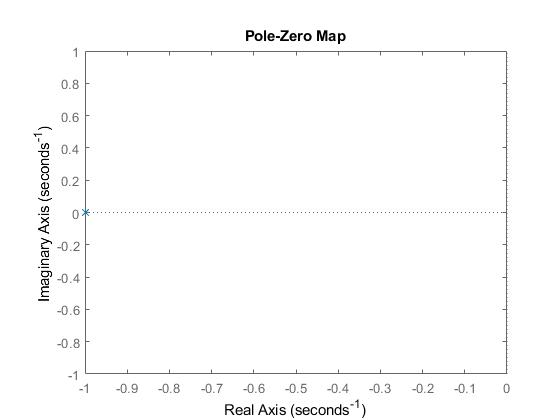
\includegraphics{Imagens/Lab2/tau1.jpg}

Como o polo da função de transferência se encontra na SPE, conclui-se que o sistema se compartará de uma forma estável.

\hypertarget{parte-2}{%
\paragraph{Parte 2}\label{parte-2}}
\addcontentsline{toc}{paragraph}{Parte 2}

Para \(\tau = 0.5\), temos a função de transferência dada por
\[
G(S)= \frac {1}{0.5s+1}.
\]

O código implementado no \texttt{Matlab} foi o apresentado abaixo.

\begin{Shaded}
\begin{Highlighting}[]
\NormalTok{g = tf([}\FloatTok{1}\NormalTok{], [}\FloatTok{0.5} \FloatTok{1}\NormalTok{])}
\NormalTok{[p, z] = pzmap(g)}
\NormalTok{pzmap(g)}
\end{Highlighting}
\end{Shaded}

Tendo como resultados de polos e zeros:

\begin{verbatim}
p =

    -2


z =

  0×1 empty double column vector
\end{verbatim}

Ou seja, a função de transferência não apresenta zeros e tem seu polo em \(s = -2\). A sua posição no plano é apresentada na figura abaixo

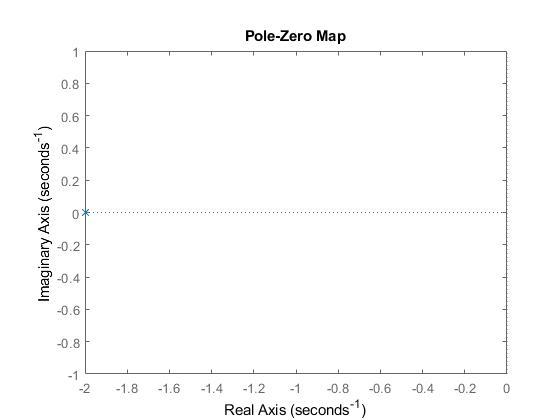
\includegraphics{Imagens/Lab2/tau2.jpg}

Como o polo da função de transferência se encontra na SPE, conclui-se que o sistema se compartará de uma forma estável. Também é possível concluir que o sistema alcanraça a estabilidade mais rápido para \(\tau = 0.5\).

\hypertarget{parte-3}{%
\paragraph{Parte 3}\label{parte-3}}
\addcontentsline{toc}{paragraph}{Parte 3}

A simulação do sistema implementada em \texttt{Matlab} está apresentado na figura abaixo.

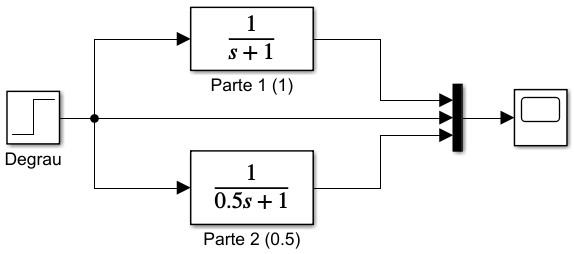
\includegraphics{Imagens/Lab2/sim1.jpg}

O resultado apresentado pelo \emph{scope} é apresentado na figura abaixo.

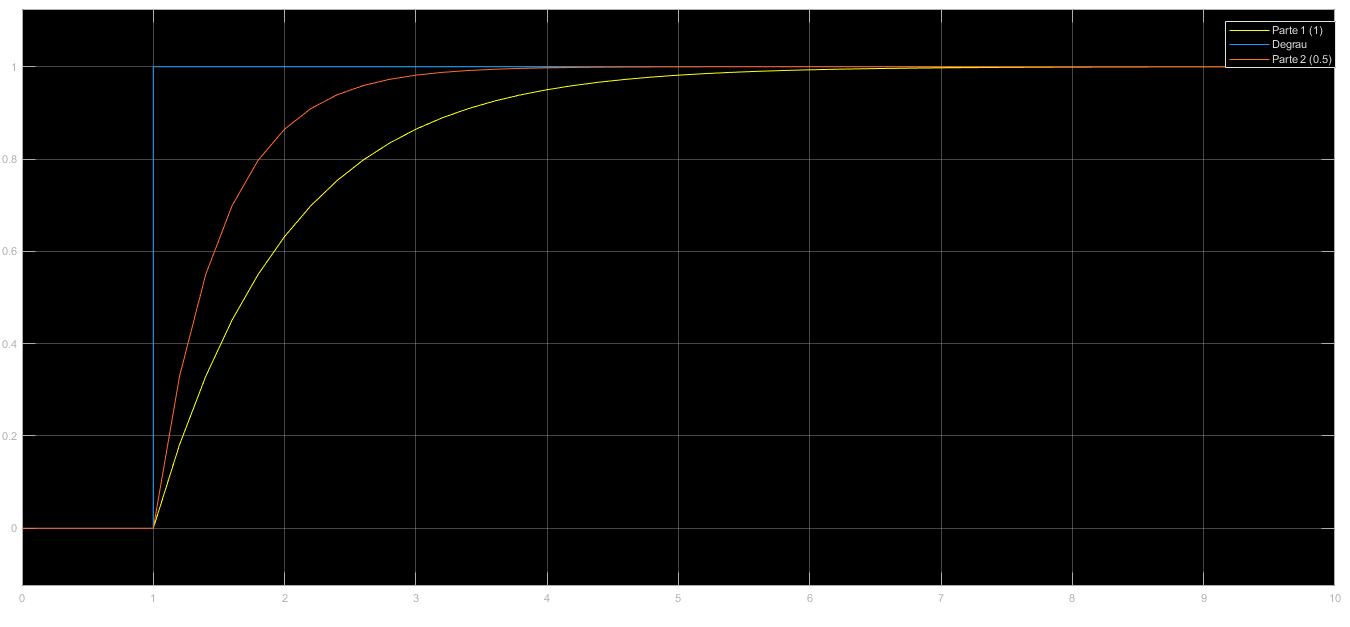
\includegraphics{Imagens/Lab2/resultSim1.jpg}

Percebe-se que, assim como esperado, o sistema se comporta de forma estável e tem uma convergência mais rápida para \(\tau = 0.5\).

\hypertarget{parte-4}{%
\paragraph{Parte 4}\label{parte-4}}
\addcontentsline{toc}{paragraph}{Parte 4}

Para a última etapa temos a função de transferência dada por
\[
G(S)= \frac {1}{s-1}.
\]

O código implementado no \texttt{Matlab} foi o apresentado abaixo.

\begin{Shaded}
\begin{Highlighting}[]
\NormalTok{g = tf([}\FloatTok{1}\NormalTok{], [}\FloatTok{1}\NormalTok{ -}\FloatTok{1}\NormalTok{])}
\NormalTok{[p, z] = pzmap(g)}
\NormalTok{pzmap(g)}
\end{Highlighting}
\end{Shaded}

Tendo como resultados de polos e zeros:

\begin{verbatim}
p =

    1


z =

  0×1 empty double column vector
\end{verbatim}

Ou seja, a função de transferência não apresenta zeros e tem seu polo em \(s = 1\). A sua posição no plano é apresentada na figura abaixo

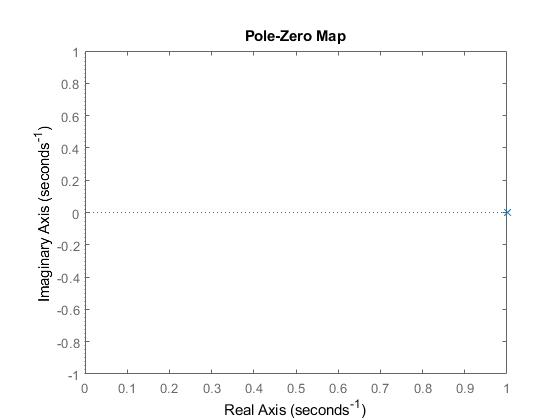
\includegraphics{Imagens/Lab2/tau3.jpg}

Como o polo da função de transferência se encontra na SPD, conclui-se que o sistema se compartará de uma forma instável. A simulação em \texttt{Matlab} está apresentada na figura abaixo.

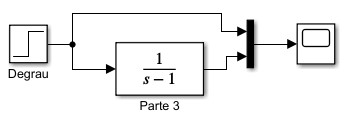
\includegraphics{Imagens/Lab2/sim2.jpg}

O resultado apresentado pelo \emph{scope} é apresentado na figura abaixo.

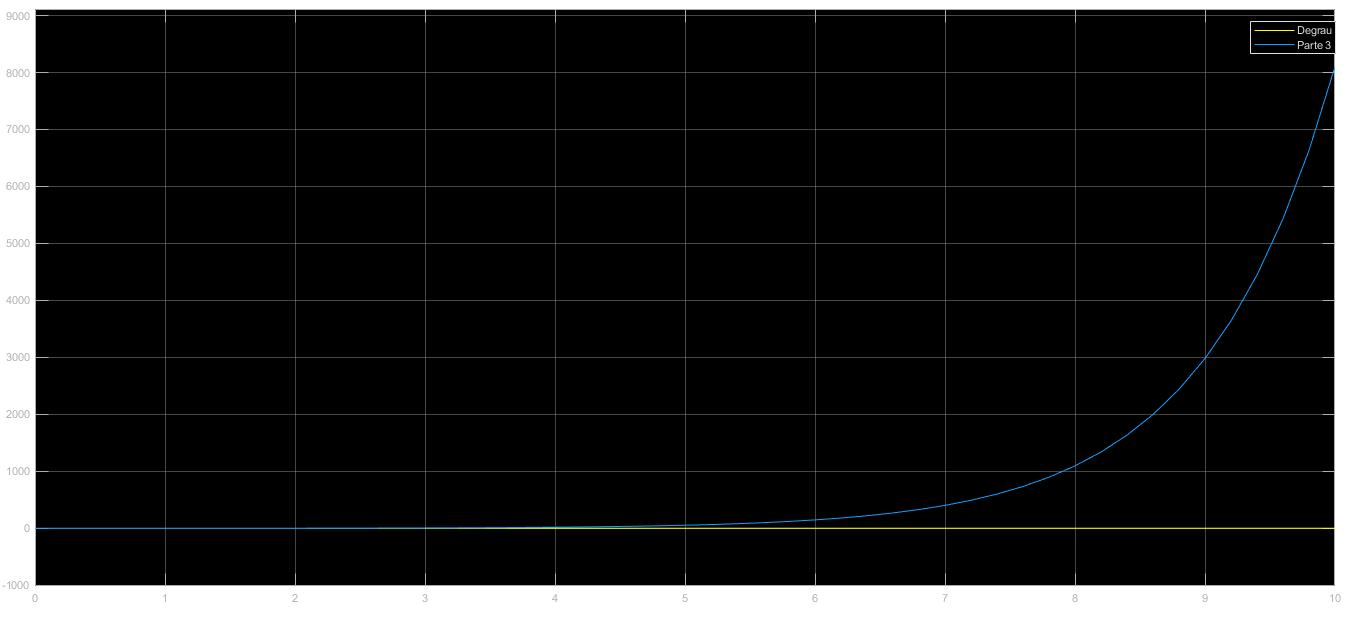
\includegraphics{Imagens/Lab2/resultSim2.jpg}

O resultado comprova o esperado. O sistema se comporta de forma instável para a função de transferência dada por \(G(s) = \frac {1}{s-1}\).

\hypertarget{identificauxe7uxe3o-de-sistemas}{%
\chapter{Identificação de Sistemas}\label{identificauxe7uxe3o-de-sistemas}}

Working on it :)

\hypertarget{applications}{%
\chapter{Applications}\label{applications}}

Some \emph{significant} applications are demonstrated in this chapter.

\hypertarget{example-one}{%
\section{Example one}\label{example-one}}

\hypertarget{example-two}{%
\section{Example two}\label{example-two}}

  \bibliography{book.bib,packages.bib}

\end{document}
